\section{\uppercase{System and Responsibility Boundaries}}
\label{sec:system}
\noindent Figure~\ref{fig:architecture} traces the system. Public context supplies the person, offering, cutoff, windows, task family, question, and shared feature/reference definitions. A typed interface permits analytical batches, inspection of compact results, and subsequent requests or finalization. Hidden evaluator requirements never enter model context, and generated analysis code is not executed.\draftassist

\begin{figure*}[!t]
\centering
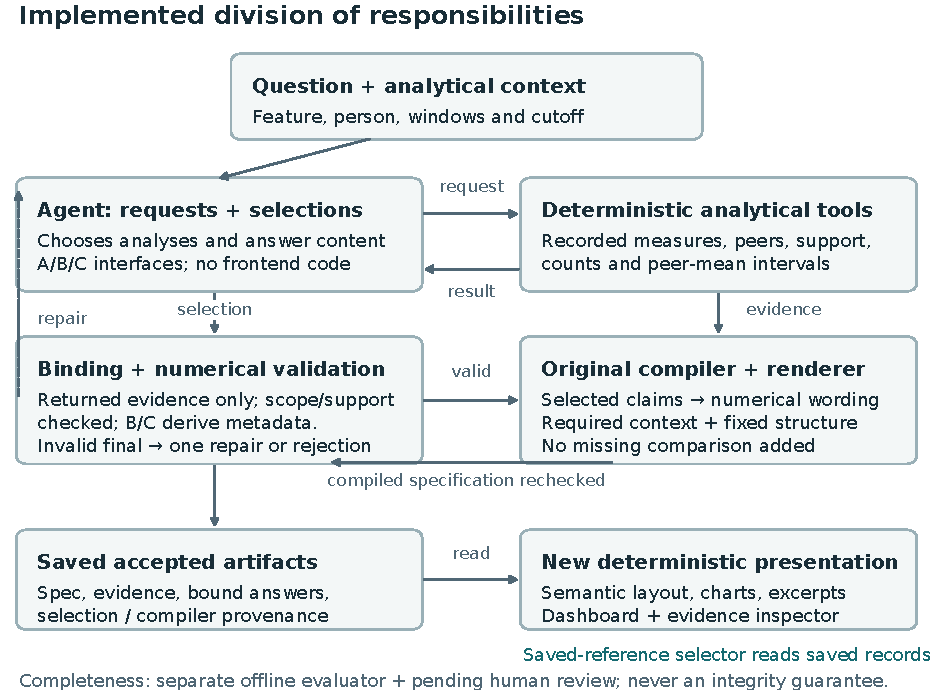
\includegraphics[width=\textwidth]{figures/architecture.pdf}
\caption{Implemented responsibilities. The agent chooses analytical requests and answer content; deterministic tools calculate values. Binding and validation can reject a final answer or permit one repair. The original compiler supplies tagged structure and context, without adding a missing comparison claim. A later presentation layer reads saved accepted artifacts; its reference selector does not call the model. Numerical validity and question completeness are checked separately.}
\label{fig:architecture}
\end{figure*}

\subsection{Evidence, Binding and Validation}
Evidence records retain features, units, focal/reference windows, counts, estimates, support, observation/assessment states, uncertainty, source/configuration hashes, seeds, and execution metadata. Model context omits raw rows; full evidence remains available for inspection.

A peer answer has analytical identity
\begin{equation}
I_{\mathrm{peer}}=(i,o,t,f,W_f,g,W_g),
\end{equation}
where $i$ is the focal person, $o$ the offering, $t$ the cutoff, $f$ the feature, $W_f$ the focal window, $g$ the reference definition, and $W_g$ its window. A personal-history identity instead contains
\begin{equation}
I_{\mathrm{personal}}=(i,o,t,f,W_b,W_r).
\end{equation}
Personal meaning excludes irrelevant peer definitions. Exact readable handles are generated only from returned evidence, not hidden desired answers.

Unknown, ambiguous, or altered identities fail without substitution or added analysis. Personal summaries repeated across evidence records are equivalent only if person, feature, units, cutoff, windows, means, counts, change, and support agree exactly. Resolution chooses a stable returned identifier and retains aliases; it creates no peer answer.

Validation reconstructs expectations from the trusted development bundle, checking summaries, trajectories, counts, interval endpoints, units, references, windows, eligibility, and cutoff. A recomputed content hash cannot legitimize mutated values. Numerical text binds to validated fields; unsupported scope or identifiers fail despite valid JSON. This establishes fidelity to the implementation, not scientific adequacy or question completeness.

\subsection{Compiler and Provenance}
The vocabulary comprises peer comparison, personal change, assessment status, observation status, and measurement limitation. Peer selections produce comparison claims/panels; personal selections produce personal claims/trajectories. Support rules yield descriptive or scoped-insufficiency wording. Unknown grades remain unavailable measurements.

The common contract supplies required trajectories, observation/assessment context, and qualifications, but no missing comparison or personal claim. Supplied timelines or grade limitations can nevertheless answer a requested item. Provenance separates selections, resolutions, metadata, and compiler additions. Every number is calculated and inserted deterministically: ``model-selected'' means chosen content, never model-authored arithmetic.

\subsection{Adaptive Presentation of Saved Answers}
Publication views postdate the experiment and reorganize saved content without new evidence, changed windows, repaired omissions, or rescoring. Layout follows semantics, not case identifiers. Exact personal duplicates may collapse with checked equivalence and preserved multiplicity; distinct peer claims remain in expanded views. Completeness is judged from full original dashboards, not publication crops.

Figure~\ref{fig:adaptation} contrasts a personal trajectory with a selected peer comparison against a view of recorded zeros, ineligibility, and unavailable quantities. The original compiler supplied the latter's observation timeline and grade context; presentation did not discover them. Assessment views instead emphasize observed-week submission measures and dated states. All views provide an expandable evidence inspector and source-method information.

\begin{figure*}[!t]
\centering
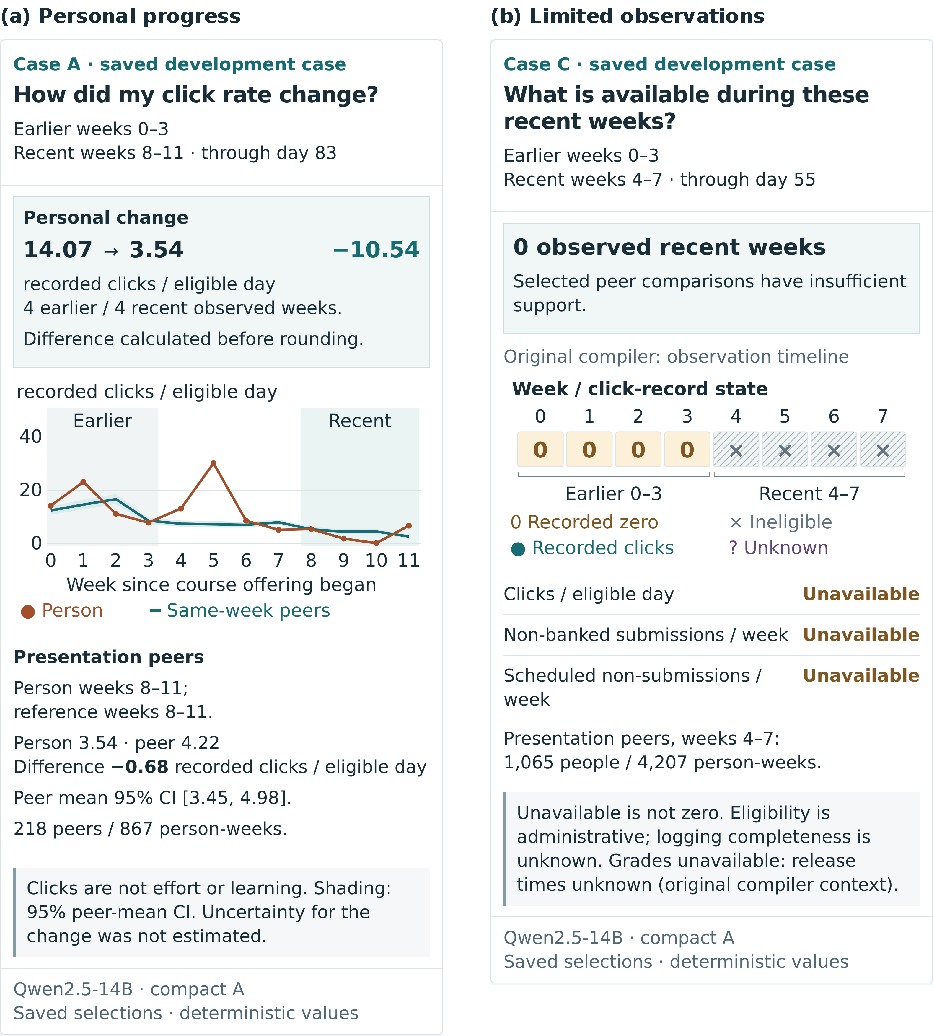
\includegraphics[width=\textwidth]{figures/adaptation.pdf}
\caption{New renderings of saved development answers from compact condition A. (a) Case 01: selected personal change and recent-peer context. The unrounded means produce the displayed change; the shaded band is a pointwise 95\% peer-mean bootstrap interval, not uncertainty for personal change. (b) Case 09: recorded zero activity is distinct from ineligibility and unavailable recent quantities. This answer was accepted after one historical repair; its original compiler supplied the observation timeline and grade-availability context. Anonymous display aliases differ from experimental condition labels. Deterministic presentation adaptation establishes neither improved accuracy nor usability.}
\label{fig:adaptation}
\end{figure*}

Reference comparisons use aligned scales and explicit focal and reference windows. In Figure~\ref{fig:reference}, a working selector switches between two comparisons already selected by the same agent. It updates the highlighted result, counts, labels, chart, and evidence link together. The focal measurement stays fixed while the reference period changes. This is viewing saved analysis, not a new investigation or statistical recomputation. Full and excerpted views retain the distinction between unavailability and zero, and peer-mean intervals are not repurposed as uncertainty for a contrast.
